%\addcontentsline{toc}{chapter}{ПРИЛОЖЕНИЕ А}
\StructuredChapter{ПРИЛОЖЕНИЕ А}

%\begin{figure}[h!] %Как сделать скрин в векторе или более качественно показать логи?
%	\centering
%	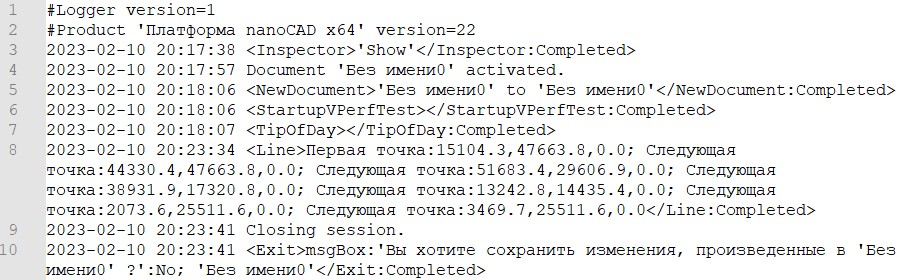
\includegraphics[width=1\textwidth]{inc/img/logs2.jpg}
%	\caption{Пример логов NanoCAD}
%	\label{NanoCAD_logs}
%\end{figure}
%
%\StructuredChapter{ПРИЛОЖЕНИЕ Б}

\begin{lstinputlisting}[
	caption={Класс LogReader},
	label={LogReader.h},
	language=C++,
	]{./inc/src/LogReader.h}
\end{lstinputlisting}

\newpage
\begin{lstinputlisting}[
	caption={Класс DataBase},
	label={DataBase.h},
	language=C++,
	]{./inc/src/DataBase.h}
\end{lstinputlisting}

\newpage
\begin{lstinputlisting}[
	caption={Класс Calculator},
	label={Calculator.h},
	language=C++,
	]{./inc/src/Calculator.h}
\end{lstinputlisting}

\StructuredChapter{ПРИЛОЖЕНИЕ Б}

\begin{figure}[h!]
	\centering
	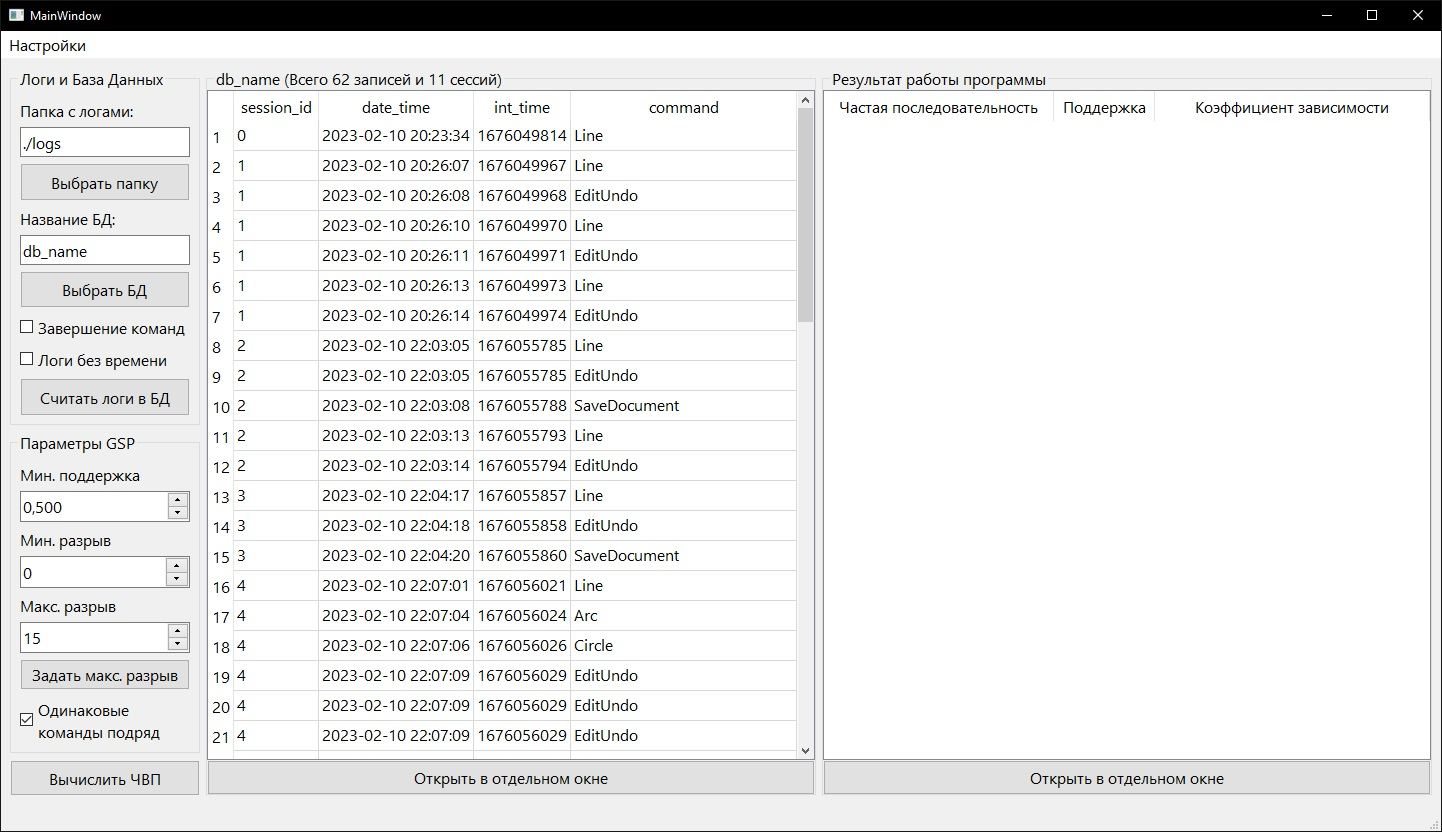
\includegraphics[width=1\textwidth]{inc/img/interface1.jpg}
	\caption{Интерфейс программы 1}
	\label{interface1}
\end{figure}

\begin{figure}[h!]
\centering
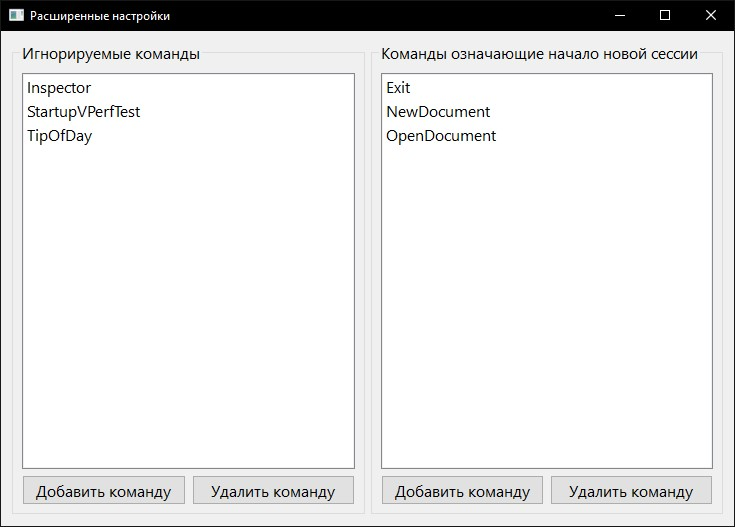
\includegraphics[width=0.9\textwidth]{inc/img/interface2.jpg}
\caption{Интерфейс программы 2}
\label{interface2}
\end{figure}

%\newpage
%\begin{figure}[h!] %Как сделать скрин в векторе или более качественно показать пример работы программы?
%	\centering
%	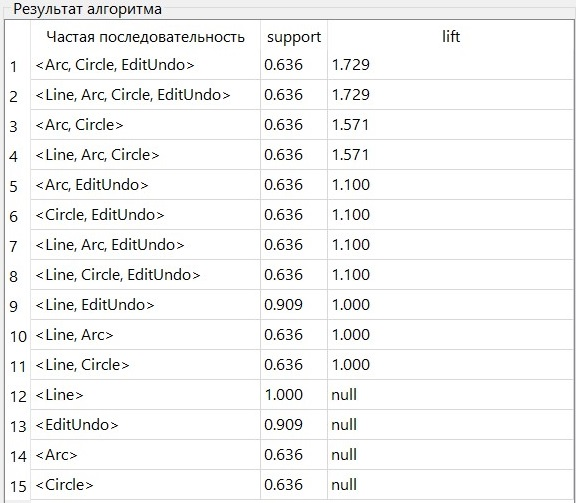
\includegraphics[width=1\textwidth]{inc/img/example1.jpg}
%	\caption{Пример работы программы 2}
%	\label{example1}
%\end{figure}
%
%\newpage
%\begin{figure}[h!]
%	\centering
%	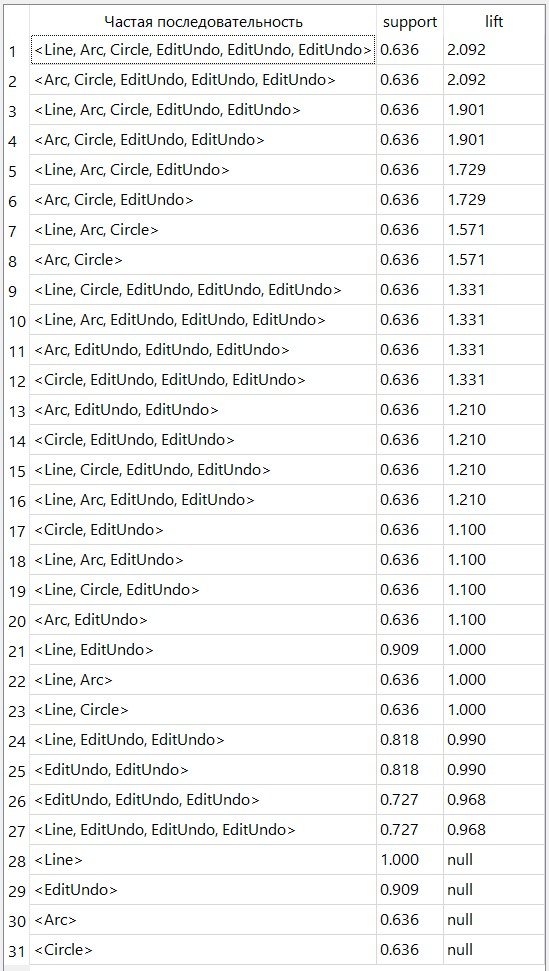
\includegraphics[width=0.8\textwidth]{inc/img/example2.jpg}
%	\caption{Пример работы программы 2}
%	\label{example2}
%\end{figure}

%\StructuredChapter{ПРИЛОЖЕНИЕ Г}
%
%\begin{center}
%Презентация
%\end{center}